De NOR\index{NOR} geeft aan dat beide ingangen 0 zijn, als dat het geval is dan is de uitgang 1.

\rowcolors{2}{gray!10}{gray!20}
\begin{tabular}{ |c|c|c| }
\hline
\rowcolor{gray!60}
	Input 1 & Input 2 & Output \\
	\hline
	0 & 0 & 1 \\
	\hline
	0 & 1 & 0 \\
	\hline
	1 & 0 & 0 \\
	\hline
	1 & 1 & 0 \\
	\hline
\end{tabular}

Het symbool voor de NOR is weergegeven in figuur \ref{symbool:nor}

\begin{figure}[h]
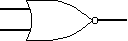
\includegraphics{nor_symbool}
\centering
\caption{Symbool van een NOR}
\label{symbool:nor}
\end{figure}

De NOR wordt gebouwd door gebruik te maken van twee transistoren die parallel aan elkaar staan, de beide basis vormen de ingang en er is een weerstand (figuur \ref{circuit:nor}.

\begin{figure}[h]
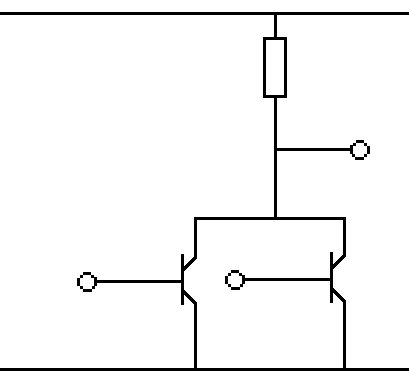
\includegraphics{nor_circuit}
\centering
\caption{NOR circuit}
\label{circuit:nor}
\end{figure}

De NOR-technologie kan je tegen komen in flash memory.

